\section{Methodology}
\label{sec:methodology}

\subsection{General Overview of Our IR System}
In the development of our \ac{IR} system, we followed the traditional \textit{Y model}, represented in the figure below.

\begin{figure}[!h]
    \centering
    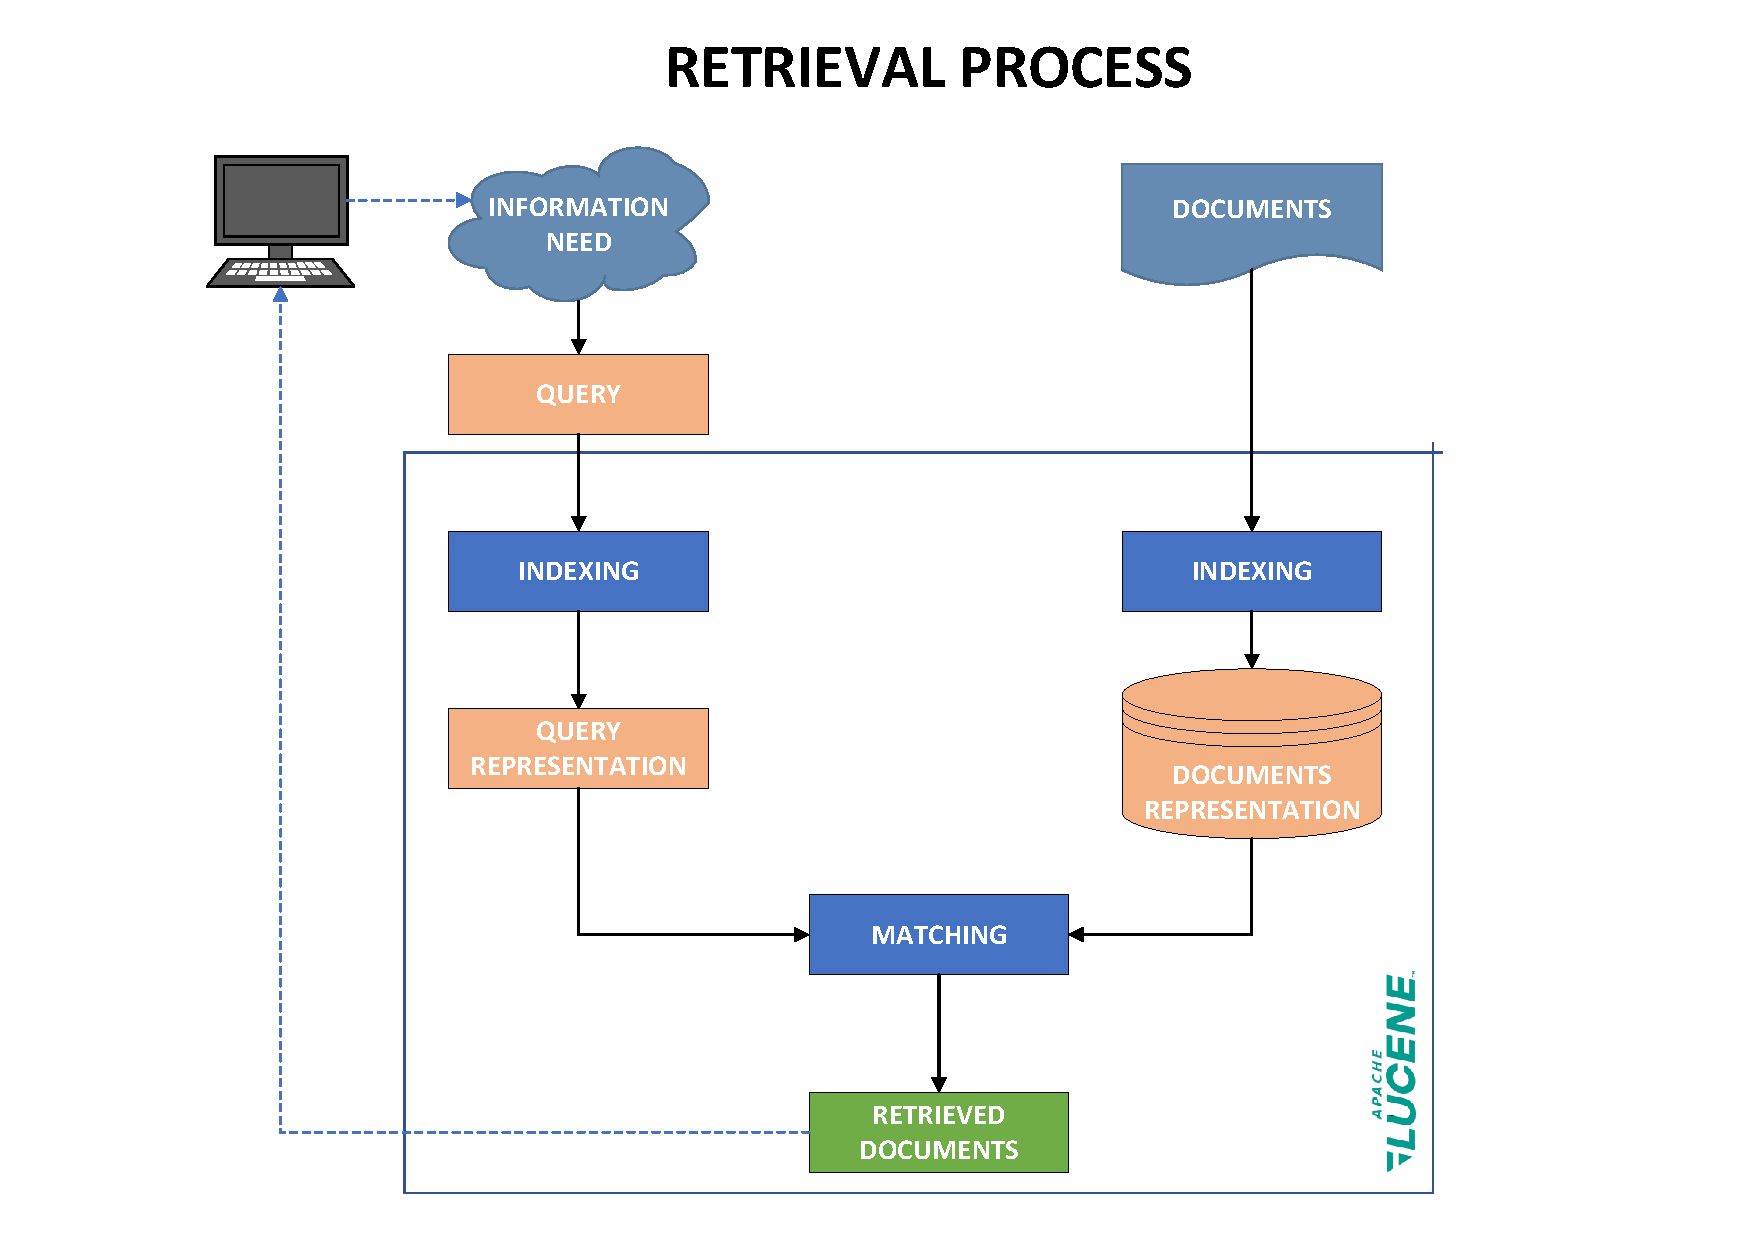
\includegraphics[width=0.9\linewidth]{figure/Y.pdf} 
    \caption{Apache Lucene Y Model.}
    \label{fig:lucene_yModel}
\end{figure}

The workflow of our system, starting from the train collection provided by \textit{LongEval} \cite{cleflongeval}, is as follows:
\begin{enumerate}
    \item \textbf{Parsing}: The first phase consists of parsing the documents in the collection, which is a pre-processing operation performed to clean them from unnecessary noises. Since the collection is composed of web pages, the documents contain many leftovers like JavaScript scripts, HTML and CSS codes, HTTP and HTTPS URIs, and so on. The purpose of this phase is to ease the processing performed in the following phases.

    \item \textbf{Indexing}: Each parsed document is then analyzed and indexed keeping only the necessary information. Indexed documents are composed of two fields: an \textit{id} field, containing the identifier of the document in the collection, and a \textit{content} field, containing the entire body of the document cleaned by the parsing and indexing phases.

    \item \textbf{Query Formulation}: Topics are then parsed using the same analyzer used for documents, and used to formulate queries. For each topic, together with the already provided query, around 15 others query variants are generated (through GPT model) by us and used altogether for searching relevant documents.

    \item \textbf{Re-ranking}: The retrieved documents are re-ranked combining the scores obtained with two different approaches which compute the similarity of the document to the query given in the topic.

\end{enumerate}

\begin{figure}[!h]
    \centering
    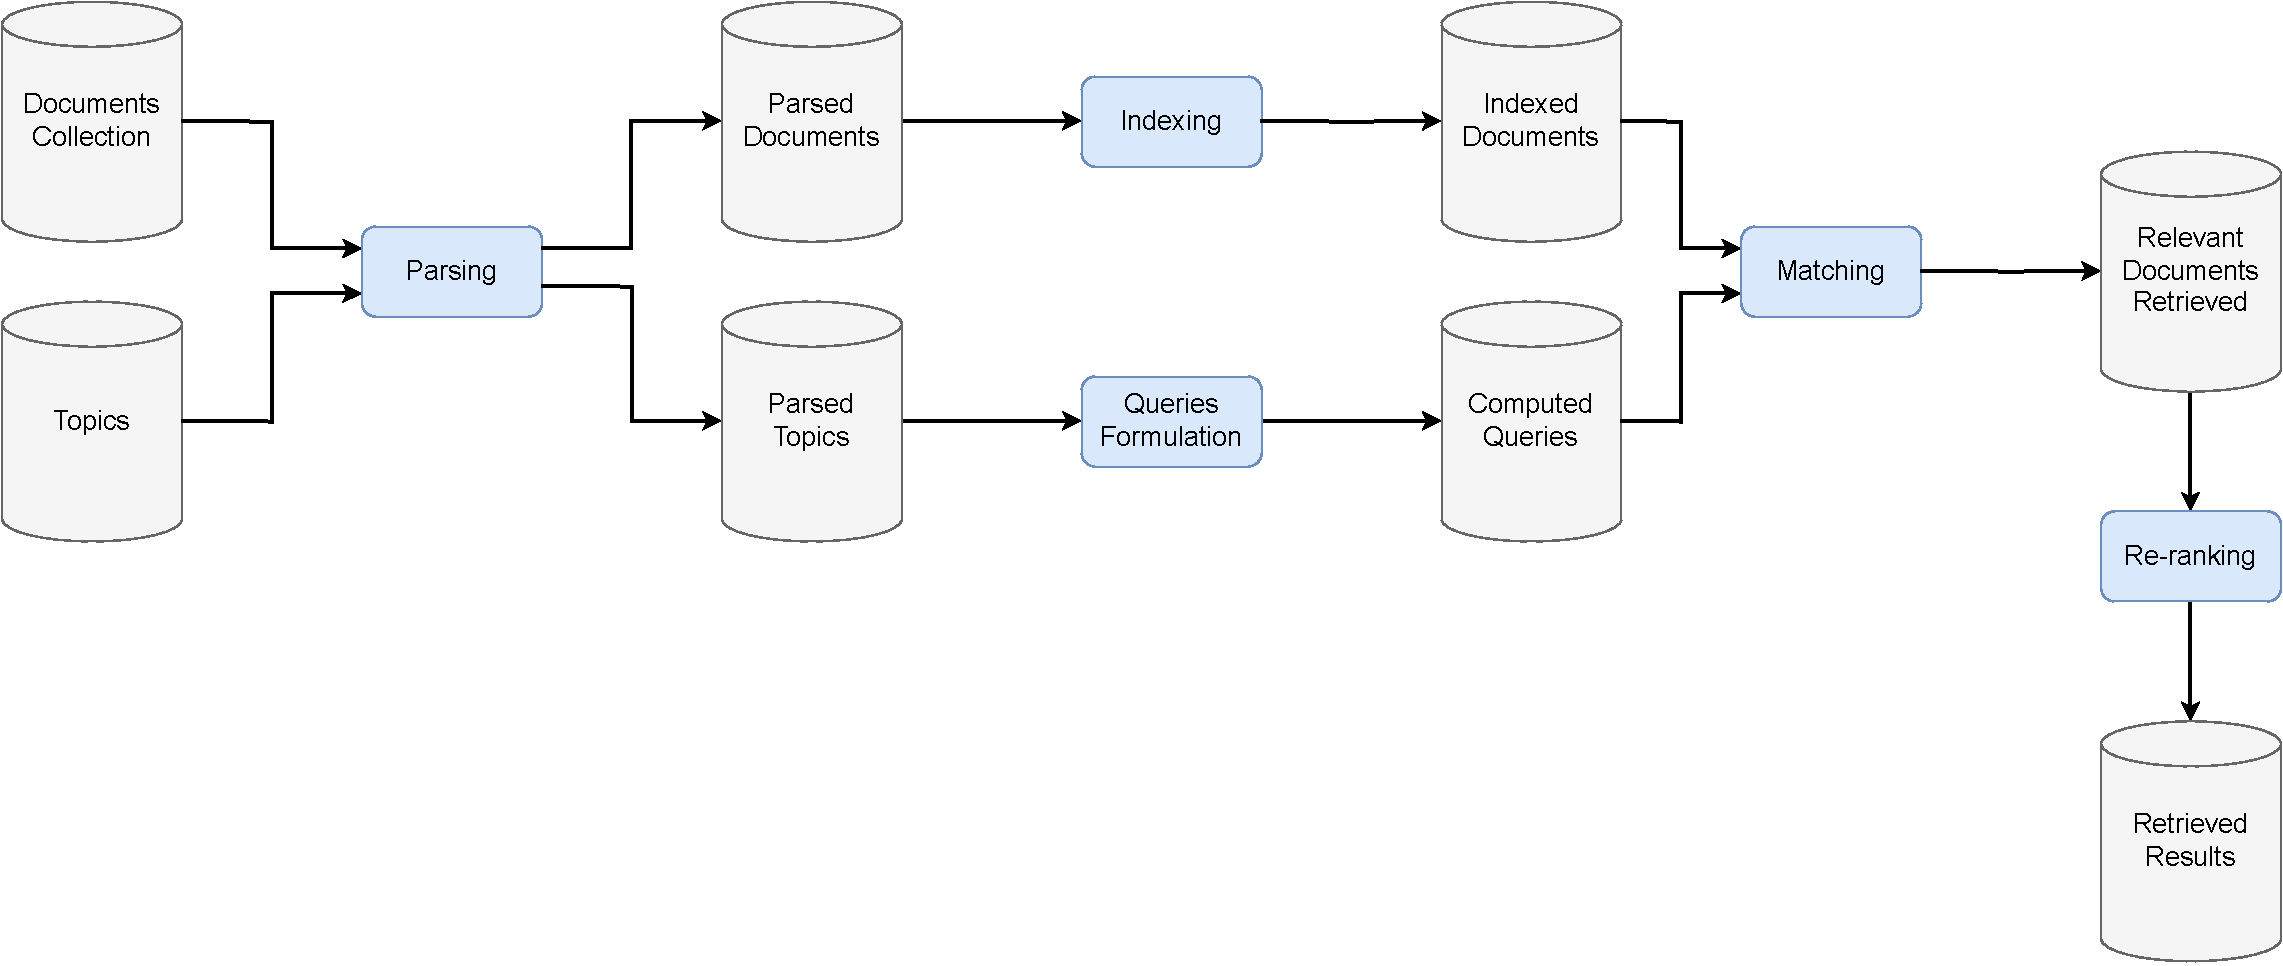
\includegraphics[width=\textwidth, height=\textheight, keepaspectratio]{figure/CLOSE_IR_Workflow (2).pdf}
    \caption{Workflow of the IR system implemented by \textit{CLOSE}.}
    \label{fig:CLOSE_IR_Workflow}
\end{figure}

\newpage
\enlargethispage{5\baselineskip}
\subsection{Class Diagram}

\begin{figure}[!h]
    \centering
    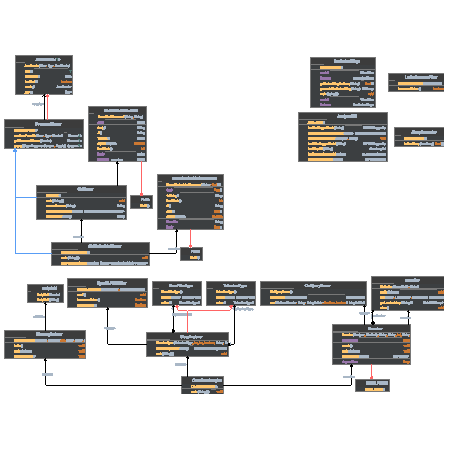
\includegraphics[height=0.7\textheight, angle =90, keepaspectratio]{figure/Classes_diagram_white_crop.pdf}
    \caption{Diagram of the classes implemented by \textit{CLOSE} \ac{IR} system}
    \label{fig:Classes_diagram_white}
\end{figure}
\clearpage
The class diagram of the system [\ref{fig:Classes_diagram_white}] retraces the Y model [\ref{fig:lucene_yModel}] of an IR system: in fact, it is possible to see as an indexer class and a searcher class that are, in this order,
called by the main class \textit{CloseSearchEngine} of our system. The \textit{Analyzer} class is instantiated before all, as it is used both from the two main branches stated before. Here many other Lucene (and Solr for NLP filters trials) tool are istantiated, as long as this component
is responsible of analyzing tokens, and here most of our processing phase goes on: in particular, the tokenizer and the stemmer (and some NLP filters used in a trial).\\
The other connected component of the diagram is related to the parsing section: here, while walking on the file tree, the \textit{Indexer} uses this component to generate, from a JSON document, an actual Java object (\textit{ParsedTextDocument}) representing it with its fields.\\
The \textit{Searcher} class firstly parses the queries from the trec format in a Lucene \textit{QualityQuery} object, through our \textit{ClefQueryParser} class. It also istantiate the \textit{ReRanker}, responsible of the second ranking phase.\\
Other utility classes are included but no longer used in our project.

\subsection{Parser} \label{parser_subsec}
As stated before, the documents in the collection provided by the \ac{CLEF} \textit{LongEval LAB 2023} \cite{cleflongeval} are essentially the corpus of web pages, to better represent the nature of a web test collection.
From this, the need for performing a pre-processing phase of parsing the documents before analyzing and indexing them arises.
In this phase, the documents are cleaned from all the residuals of codes not useful for our purposes. 
We first created an abstract class \textit{DocumentParser} and then extended it by implementing a custom \textit{ClefParser} class, which contains many functions for removing sundry types of noises that can be present in documents. 
This was the result of the trial and error approach we adopted for implementing this class:
\begin{itemize}
\item We started by our own read of a large statistical sample size of the documents in the collection to decide which types of noises needed to be removed.
\item Then we implemented the parser and ran it.
\item The results of the parsing were stored, and a sample of the parsed documents was analyzed to start this procedure again.
\end{itemize}

\begin{figure}[!h]
    \centering
    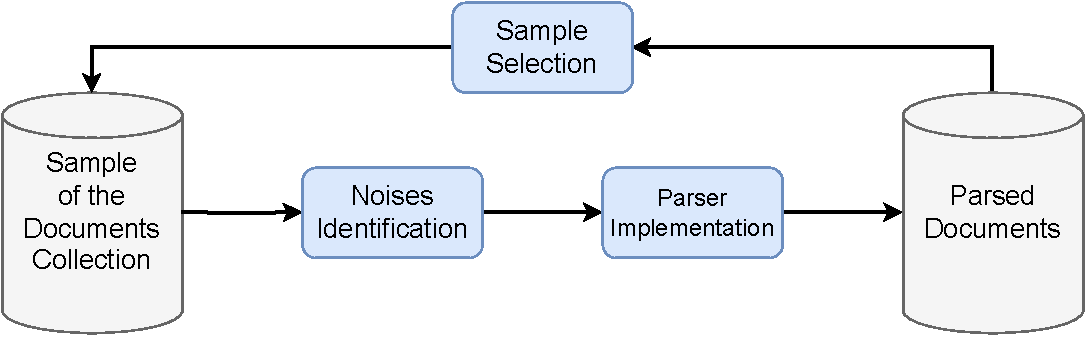
\includegraphics[width=0.8\linewidth]{figure/Parser_implementation_workflow.pdf}
    \caption{Workflow of the parser implementation.}
    \label{fig:Parser_implementation_workflow}
\end{figure}

The types of noises we tried to remove are the following:
\begin{itemize}
\item \textit{JavaScript} scripts,
\item \textit{HTTP} and \textit{HTTPS} URIs,
\item \textit{HTML} tags and \textit{CSS} stylesheets,
\item \textit{XML} and \textit{JSON} codes,
\item Meta tags and document properties,
\item Navigation menus,
\item Advertisements,
\item Footers,
\item Social media handlers,
\item Hashtags and mentions.
\end{itemize}
The final decision about the type of noises to effectively remove for our runs was the most crucial part of this process. \\
For establishing this we used a trial \& error approach, and at the end we decided to remove only the \textit{JavaScript} scripts and the \textit{HTTP} and \textit{HTTPS} URIs. Regarding \textit{URI}s, although these are usually important because they can contain valuable keywords, we noticed an improvement in \ac{MAP} of almost 0.5 points by just removing them. \\
We also identified some patterns of words and symbols to remove:
\begin{itemize}
\item Two words separated by an underscore, like \textit{word1\_word2}
\item Two words separated by a colon, like \textit{word1:word2}
\item Two words separated by a point, like ``\textit{word1.word2}''
\end{itemize}
We used \textit{Regular Expressions} \cite{regexdefinition} to identify and remove these patterns.  

The structure of the parsed document is defined in the \textit{ParsedTextDocument} class, and it is composed of just two fields, as provided by \ac{CLEF}:
\begin{enumerate}
\item \textit{id}: the identifier of the document,
\item \textit{body}: the (parsed) content of the document.
\end{enumerate}
The constructor of \textit{ParsedTextDocument} is the following:
\begin{lstlisting}[language=Java]
    /**
     * Creates a new parsed document.
     *
     * @param id  the document identifier.
     * @param body the document body.
     */
    public ParsedTextDocument(final String id, final String body) 
\end{lstlisting}
Inside it, multiple controls about the validity and integrity of the parameters are performed, then an object of the class is instantiated. 


\subsection{Analyzer} \label{analyzer_subsec}
The Analyzer is responsible for analyzing the extracted documents and preparing them for the Indexing and Searching phases. 
It does so by combining a series of techniques of text processing such as tokenization, stemming, stopword removal, and many more.\\
We extended Apache Lucene's Analyzer abstract class \cite{luceneanalyzer} by creating a custom class \textit{CloseAnalyzer}, which is fully customizable by its parameters that can be chosen when creating an instance of the class. 
This has been done because we tried different settings and approaches to maximize the results and kept all the possible variations as optional settings.
This \textit{CloseAnalyzer} is passed as a parameter and then used by the \textit{DirectoryIndexer} and by the \textit{Searcher}. \\
The constructor of \textit{CloseAnalyzer} accepts the following parameters:
\begin{itemize}
  \item \textbf{tokenizerType}: used to choose between three standard \textit{Lucene} tokenizers: \textit{WhitespaceTokenizer} \cite{lucenetokenizer}, \textit{LetterTokenizer} \cite{lucenelettertokenizer}, and \textit{StandardTokenizer} \cite{lucenestandardtokenizer}.
  
  \item \textbf{stemFilterType}: the possible choices for the stemming types are four standard \textit{Apache Solr} \cite{solr} filters: \textit{EnglishMinimalStemFilter} \cite{solrminimalstemfilter}, \textit{KStemFilter} \cite{solrkstemfilter}, \textit{PorterStemFilter} \cite{solrporterstemfilter}, and \textit{FrenchLightStemFilter} \cite{solrfrenchlightstemfilter}. 
  We also tried using \textit{FrenchMinimalStemFilter} \cite{solrfrenchminimalstemfilter} and a custom filter called \textit{LovinsStemmerFilter} based on a LovinsStemmer \cite{lucenelovinsstemmer} implementation but decided to keep them commented as they didn't improve the results.
  
  \item \textbf{minLength} and \textbf{maxLength}: these are integers that simply specify the minimum and maximum length of a token, applying Lucene's \textit{LengthFilter} \cite{lucenelengthfilter}.
  
  \item \textbf{isEnglishPossessiveFilter}: specifies whether to use Lucene's \textit{EnglishPossessiveFilter} \cite{luceneenglishpossessivefilter} or not. 
  Of course, this can be useful when operating with the English dataset.
  
  \item \textbf{stopFilterListName}: with this parameter, it's possible to insert the path of an eventual word stoplist \textit{.txt} file located in the \textit{resources} folder. 
  To do this we use Lucene's \textit{StopFilter} \cite{lucenestopfilter} and a custom class called \textit{AnalyzerUtil} that uses a \textit{loadStopList} method to read and load all the stoplist words from the specified file. 
  The stoplists we created are based on the standard ones but modified after inspecting the index with the \textit{Luke} \cite{luke} tool. 
  We have lists of different lengths and different ones for French and English.
  
  \item \textbf{Character nGramFilterSize}: if specified, this parameter is used to define the size of the n-grams to be applied by Lucene's \textit{NGramTokenFilter} \cite{lucenengramtokenfilter}.
  
  \item \textbf{Word nGramFilterSize}: similar to the previous one, if used, this integer number indicates the shingle size to be applied by Lucene's \textit{ShingleFilter} \cite{luceneshinglefilter} that allows the creation of a combination of words.
  
  \item \textbf{useNLPFilter}: this boolean allows the use of Solr's \cite{solr} \textit{OpenNLPPPOSFilter} \cite{solropennlpposfilter} for Part-Of-Speech Tagging and of a custom class called \textit{OpenNLPNERFilter} for Named Entity Recognition. 
  To load the \textit{.bin} models, which are located in the \textit{resources} folder, we use two methods from \textit{AnalyzerUtil}: \textit{loadPosTaggerModel} and \textit{loadNerTaggerModel}.
  
  \item \textbf{lemmatization}: specifies whether to use Solr's \textit{OpenNLPLemmatizerFilter} \cite{solropennlplemmafilter} by loading a \textit{.bin} model file in the \textit{resources} folder using AnalyzerUtil's \textit{loadLemmatizerModel} function.
  
  \item \textbf{frenchElisionFilter}: we applied this only when using the French dataset by adding Lucene's \textit{ElisionFilter} \cite{luceneelisionfilter} with an array of the following characters: 'l', 'd', 's', 't', 'n', 'm'.
\end{itemize}
On top of this, a \textit{LowerCaseFilter} \cite{lucenelowercasefilter} is always applied. \\
We also tried Lucene's \textit{ASCIIFoldingFilter} \cite{luceneasciifoldingfilter} and \textit{SynonymGraphFilter} \cite{lucenesynonymgraphfilter}. 
For the second one, only for the French Dataset, we used a \textit{SynonymMap} \cite{lucenesynonymmap} based on a \textit{.txt} file containing French synonyms.
\newline
After different trials with different variations of the parameter, the following is the instance of the \textit{CloseAnalyzer} we used:

\begin{lstlisting}
final Analyzer closeAnalyzer = new CloseAnalyzer(CloseAnalyzer.TokenizerType.Standard, 2, 15, false, "new-long-stoplist-fr.txt", CloseAnalyzer.StemFilterType.French, null, null, false, false, true);
\end{lstlisting}
We have opted for the French dataset and by doing so we have the \textit{StandardTokenizer}, 2 and 15 as minimum and maximum token length, we use \textit{frenchElisionFilter}, \textit{FrenchLightStemFilter}, and a list of 662 French words as a stoplist.
This stoplist has been built upon a popular French stoplist together with the most frequent stopwords in the collection.  
We didn't use any of the other parameters.
We utilized the Gson library to efficiently parse a JSON files that contained query expansions. By leveraging Gson's capabilities, we were able to seamlessly convert the JSON data into Java objects, enabling effortless manipulation and integration of the query expansions into our application.


\subsection{Searcher} \label{searcher_subsec}
The purpose of the \textit{Searcher} is to search through the indexed documents to retrieve relevant information based on user queries after analyzing them and to
return a ranked list of documents that match the user’s information needs.
\newline
Our implementation does so by accepting the following parameters:
\begin{itemize}
  \item \textbf{analyzer}: in this case, an instance of \textit{CloseAnalyzer}.
  \item \textbf{similarity}: we decided to opt for the \textit{BM25Similarity} \cite{lucenebm25similarity} function with the parameters \textit{k1} and \textit{b} tuned at 1.2 and 0.90.
  \item \textbf{Run options}: there are parameters for the index path, the topics path, the run path and the run name, the number of the expected topic (in our case 50), and the maximum number of documents retrieved (in our case 1000).
  \item \textbf{reRankModel}: this is the type of model used to do a Re-Ranking on the retrieved documents. 
  In our case, we use a model called \textit{all-MiniLM-L6-v2} \cite{huggingfaceallminilml6v2}, explained in the following subsection. 
  If the parameter is set to null, no model is used and the documents are scored normally.
\end{itemize}


\subsubsection{Query Expansion}
When running the search function, one of the first actions performed is to generate new queries from the original ones by query expansion \cite{wang2023}. \\
% For this task we have taken inspiration from the work of Shuai Wang \cite{wang2023}. 
We created a Python script that, given the \textit{*.trec} topic file, generates all the expanded terms for each query and stores everything in a \textit{.json} file called \textit{result}, containing all the expansions.
\newline
We use \textit{OpenAI's} \textit{Text completion} \cite{openaicompletionapi} endpoints to generate the expansions, we can use our need as prompt and the model will generate the result. 
We used the \textit{davinci} model, which is the most powerful one, and we set the \textit{temperature} parameter to 0.6, which is the value that gives the best results.
\newline
The sample result for prompt 
\begin{center}
    \textit{``Expand the following query with {num\_expansions} related terms or phrases for information retrieval (search-engine): {query} and the result should be in array format without any numbers at first [expanded\_term1, expanded\_term2, ...]''}     
\end{center}
is:
\begin{table}[H]
    \begin{tabular}{|l|l|l|}
        \hline
        Query                 & text-davinci-002                                                                                                                                                                  & text-davinci-003                                                                                                                                                                    \\ \hline
        antivirus comparaison & \begin{tabular}[c]{@{}l@{}}1. Antivirus software\\ 2. Antivirus protection\\ 3. Best antivirus\\ 4. Free antivirus\\ 5. Antivirus for Windows\\ 6. Antivirus for Mac\end{tabular} & \begin{tabular}[c]{@{}l@{}}1. Antivirus Reviews \\ 2. Antivirus Software \\ 3. Antivirus Protection \\ 4. Malware Protection \\ 5. Virus Scanner \\ 6. Online Security\end{tabular} \\ \hline
    \end{tabular}
    \label{tab:query_expansion}
\end{table}
The main difference between \textit{davinci-text-002} and \textit{davinci-text-003} is that the latter has been trained on a larger dataset, allowing it to generate more accurate results \cite{davincicomparison}.


\enlargethispage{2\baselineskip}
\subsubsection{Query Boosting}
Query boosting is a technique used to assign greater relevance to certain query terms or queries.\newline
We tried the following approach that seemed to improve the overall results: when building the queries in the search function of the \textit{Searcher} (\ref{searcher_subsec}), for each query, a \textit{BooleanQuery} \cite{lucenebooleanquery} is built in the following way: 
after getting the query expansions, each of them is added to the \textit{BooleanQuery} with the clause \textit{SHOULD} (meaning that at least one of them must be satisfied) and a main query is added with the clause \textit{MUST}, indicating that it must be satisfied. \\
This main query is boosted using Lucene's \textit{BoostQuery} \cite{luceneboostquery}, with a boost value tuned at 14.68 multiplied by the number of expansions. We got this value by a trial \& error approach we used to fine tune this parameter.

\subsubsection{Document Re-Ranking}
Re-Ranking is the process of ranking documents retrieved by the search function of the \textit{Searcher} (\ref{searcher_subsec}). 
To accomplish this task, we utilized sentence transformers~\cite{sentence-transformers}, a Python framework known for its state-of-the-art sentence, text, and image embeddings. 
Various models were experimented with, and the one yielding the best results was identified as \textit{all-MiniLM-L6-v2}~\cite{huggingfaceallminilml6v2}. 
This particular model aims to train sentence embedding models using a self-supervised contrastive learning objective on vast sentence-level datasets, ultimately mapping sentences and paragraphs to a dense vector space of 384 dimensions.

To generate embeddings for both the documents and query retrieved by the search function, we loaded the \textit{all-MiniLM-L6-v2} model and instantiated a \textit{SentenceTransformer} object. 
For the purpose of calculating similarity, we employed the widely used \textit{cosine similarity} formula, which computes the similarity between two vectors. The formula is defined as follows:

\begin{equation}
\text{similarity} = \frac{t \cdot d_i}{|t| |d_i|}\label{eq:similarity_equation}
\end{equation}

Here, $t$ represents the query vector, and $d_i$ denotes the vector of the $i$-th document.

Subsequently, we interpolated this similarity score with the BM25 score to improve the ranking of the documents. 
Among the different approaches we explored, the most successful one was as follows:


\begin{equation}
\text{rank} = \text{BM25\_score} \times \text{similarity} \label{eq:rank_equation}
\end{equation}

To visualize the re-ranking operation's effectiveness, we plotted the results for 50 sample queries, as depicted in Figure \ref{fig:re-ranking}.

\begin{figure}[!ht]
\centering
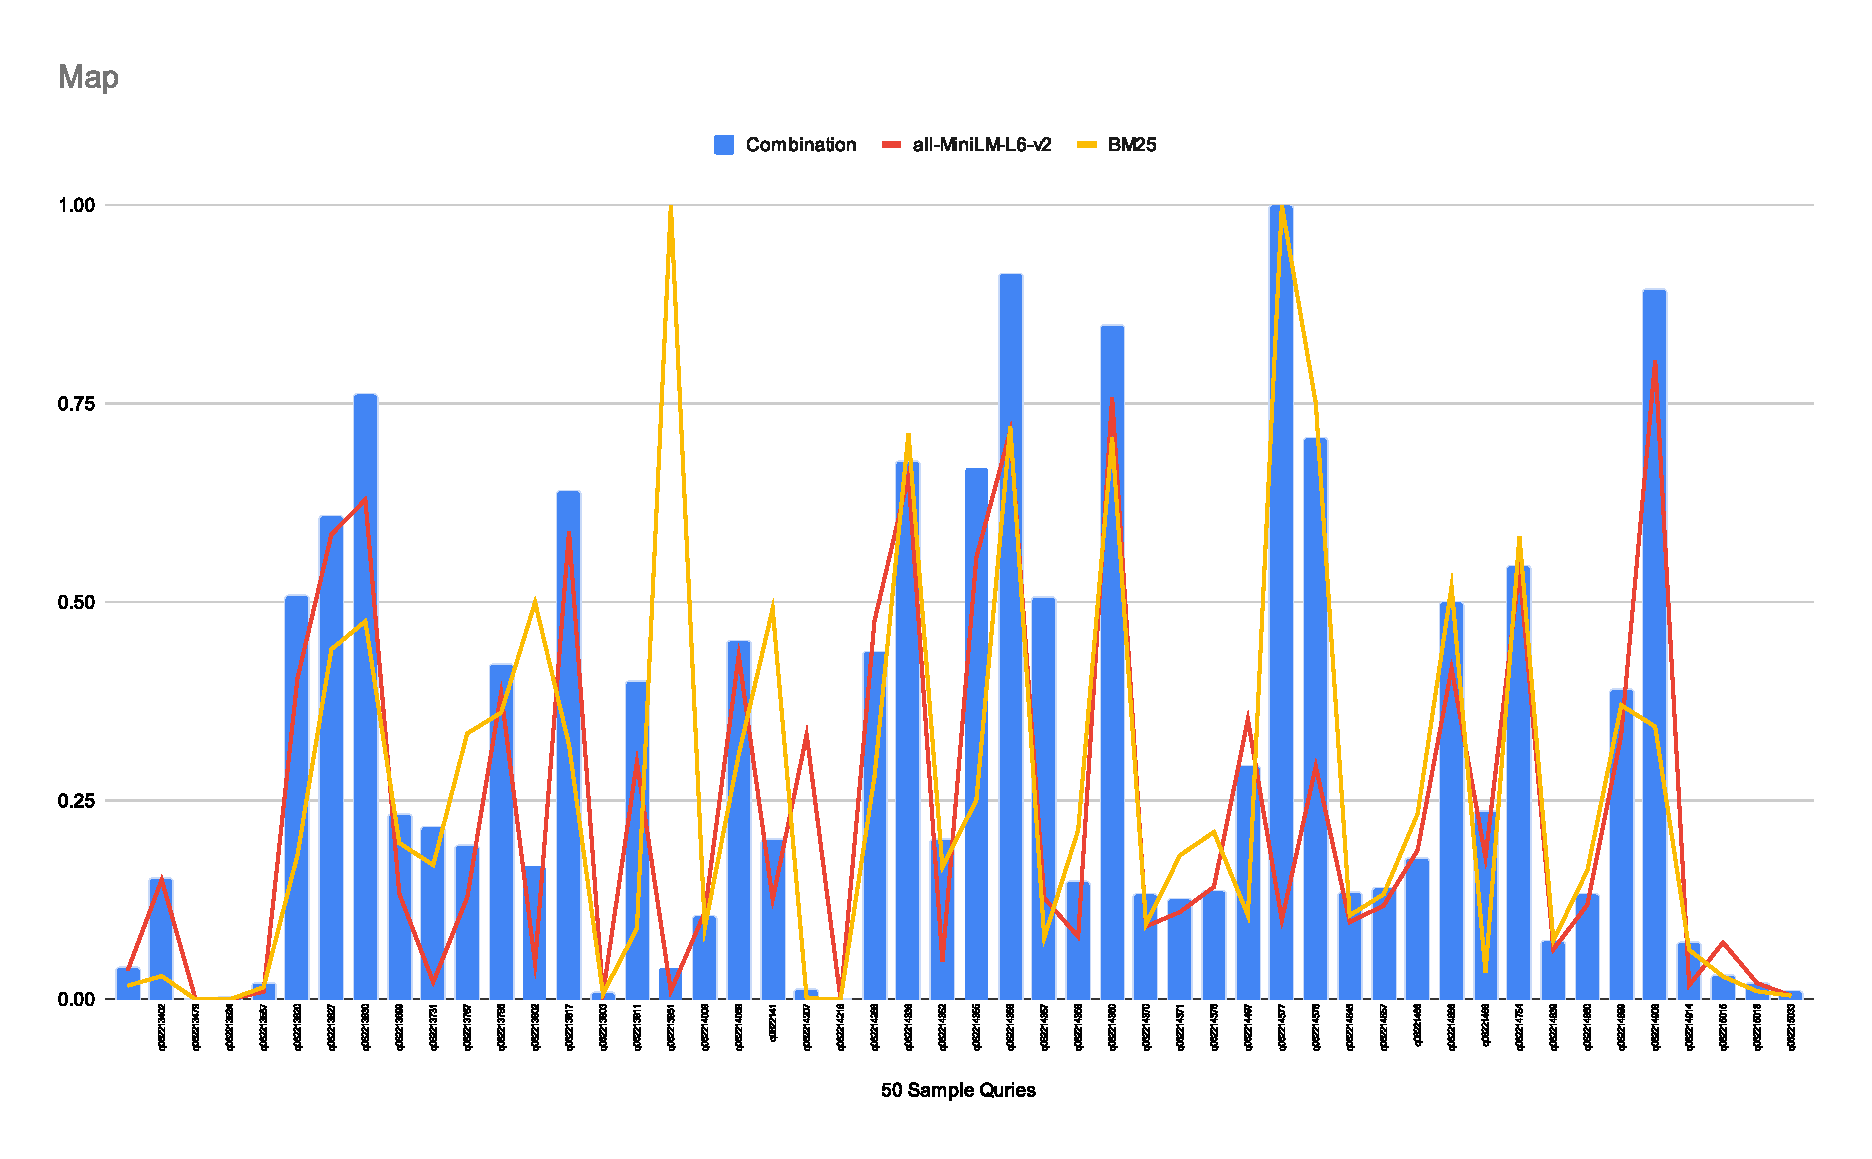
\includegraphics[scale=0.45, keepaspectratio]{figure/re-ranking}
\caption{Plot illustrating the re-ranking operation performed on 50 sample queries}
\label{fig:re-ranking}
\end{figure}

Finally, we sorted the documents based on the new rank and returned them.

